%
% File acl2014.tex
%
% Contact: giovanni.colavizza@epfl.ch
%%
%% Based on the style files for ACL-2013, which were, in turn,
%% Based on the style files for ACL-2012, which were, in turn,
%% based on the style files for ACL-2011, which were, in turn, 
%% based on the style files for ACL-2010, which were, in turn, 
%% based on the style files for ACL-IJCNLP-2009, which were, in turn,
%% based on the style files for EACL-2009 and IJCNLP-2008...

%% Based on the style files for EACL 2006 by 
%%e.agirre@ehu.es or Sergi.Balari@uab.es
%% and that of ACL 08 by Joakim Nivre and Noah Smith

\documentclass[11pt]{article}
\usepackage{acl2014}
\usepackage{times}
\usepackage{url}
\usepackage{latexsym}
\usepackage{graphicx}
\usepackage{subcaption}

%\setlength\titlebox{5cm}

% You can expand the titlebox if you need extra space
% to show all the authors. Please do not make the titlebox
% smaller than 5cm (the original size); we will check this
% in the camera-ready version and ask you to change it back.


\title{Amazon cell phone evaluation platform}

\author{Marion Kramer\\
  {\tt marion.kramer@epfl.ch} \\\And
  Alexandre Rassinoux \\
  {\tt alexandre.rassinoux@epfl.ch} \\\And
Kristina Satara \\
{\tt kristina.satara@epfl.ch} \\}

\date{18.12.2017}

\begin{document}
\maketitle
\begin{abstract}
Reviews help when making decision which product to buy, as they give possible customers personal experience and more product details. Since customers usually invest some time to studying the reviews and ratings before buying specific products from Amazon, we decided to create evaluation platform which would help the users decide about purchasing the product by giving them insight into  downsides and advantages of various brands based on the reviews. The aim of this project is to analyze reviews of different brand of Amazon cell phone products and based on the reviews to decide which of the features are important for specific brands of cell phones. For this we use natural language processing techniques, such as tf-idf matrix, ...  and Latent Dirichlet Allocation.
\end{abstract}


\section{Introduction}
Sentiment analysis, also known as opinion mining or emotion AI, is important part of natural language processing. The subject of the study is the attitude or the emotion behind certain text. The purpose of sentiment analysis is to determine weather text content is neutral, positive or negative towards some topic. 

Data used for this project is collected from Amazon, during the period of few years. Most of the data is collected between 2012 and 2014, as shown in figure 2. Each of the reviews has also ratings that are used for ground truth. The ratings are based on 5-star system, where 5 is highest and 1 is lowest rating. Distribution of the ratings is J-distribution with highest number of 5-star reviews, and it is shown in figure 1. After purchasing some of the products customers are asked to give their review and rating, which are further subject to sentiment analysis in our project. 



\begin{figure}[h!]
  \centering
    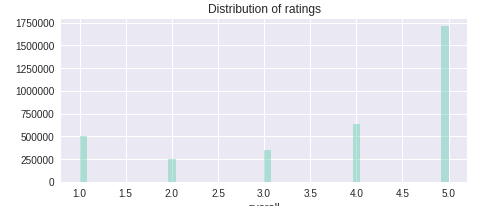
\includegraphics[width=\linewidth]{ratingDistribution.png}
  \caption{Distribution of the ratings in reviews}
  \label{fig:ratingDistribution}
\end{figure}


\begin{figure}[h!]
  \centering
    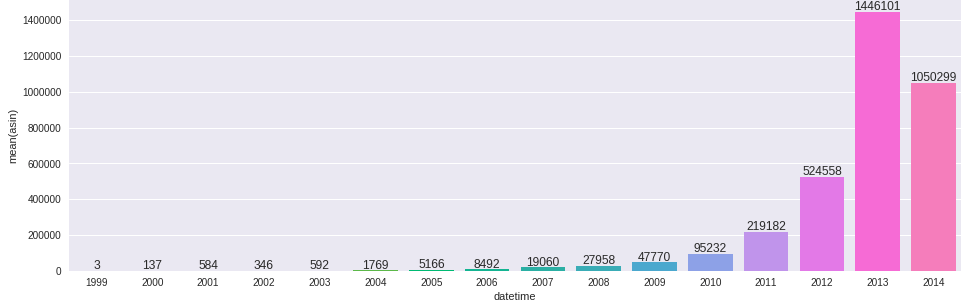
\includegraphics[width=\linewidth]{reviewsByTime.png}
  \caption{Number of reviews during time}
  \label{fig:reviewsByTime}
\end{figure}


\section{Related work}
Natural language processing is interesting and popular area of research, thus there are many papers regarding this topic. As Amazon is widely used platform, it has gained much reviews in the past few years. We focused on the cell phone reviews, and we found papers and which gave different approaches and conclusions. GIVE REFERENCES AND EXAMPLES.. In this paper they took this approach, etc etc.


\section{Data Collection}
We used dataset provided by Amazon for this project. Dataset consists of two json files - one containing the reviews, and another providing metadata about the products. We merged these two files for our further data analysis.We also transformed the data in order to improve the speed of loading and processing this dataset in our python notebook. As this dataset was incomplete, we decided to enrich it with additional dataset from Kaggle platform. This is public GSMArena dataset and it contains more than 8000 phones specifications.


\section{Dataset Description with Summary Statistics}
After merging and combining all the datasets we had, we did some decriptive statistics. Given below is the information provided in the datasets:

\begin{itemize}
  \item Reviewer's ID
  \item ID of the product reviewed
  \item Name of the reviewer
  \item Text of the review
  \item Rating given
  \item Summary of the review
  \item Time of the review
  \item Price in euros
  \item Url of the product image
  \item Brand name
  \item Category of the product
\end{itemize}

We already had some expectations,so we first explored brands of cell phone producers that our dataset contains. As expected, most of the brands were known to us. We were interested in mean and median prices of these cell phones. Figure 3. gives overview of mean prices for 25 most popular brands.   

\begin{figure}[h!]
  \centering
    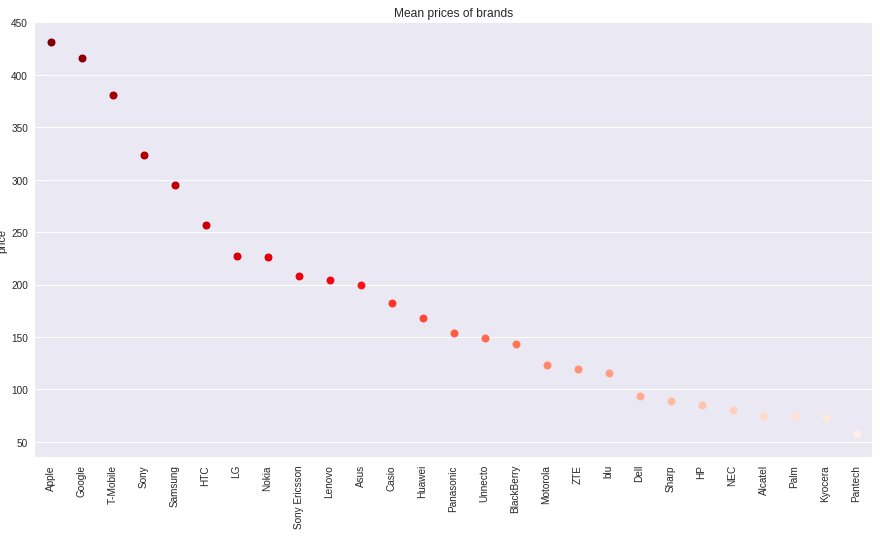
\includegraphics[width=\linewidth]{meanPrices.png}
  \caption{Mean prices per brand}
  \label{fig:meanPricePerBrand}
\end{figure}

In order to understand better our dataset and specific models contained in it, we were interested in price distribution. It is shown in Figure 4. 

\begin{figure}[h!]
  \centering
    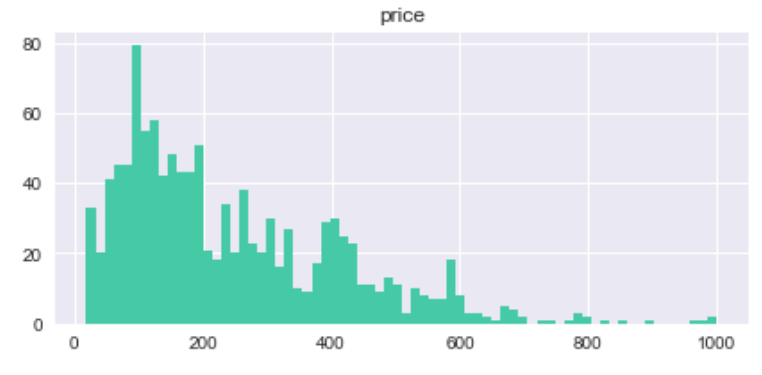
\includegraphics[width=\linewidth]{priceDistribution.png}
  \caption{Distribution of the prices}
  \label{fig:priceDistribution}
\end{figure}

Another statistics which we found interesting was average number of cell phone models per brand, mean ratings per brand, models that have highest number of the reviews. 

Customer's decision about purchasing specific model is often influenced by overall rating of the product - but in the project we show that we should be very careful when using this metric for making the decision. Not just the rating of specific model is important, but also the number of the reviews. We found during exploratory analysis that there are some models that have only a few reviews, but the rating is highest possible and there are models with average rating above four which have few thousand times more reviews. This should be taken into consideration very carefully before the decision.

We found that there are no correlations between the price and the rating. Figure 5. shows correlations of words with the ratings - either high or low rating. We notice that some words have high correlation with the reviews - for example battery and phone. 


\begin{figure}[h!]
  \centering
    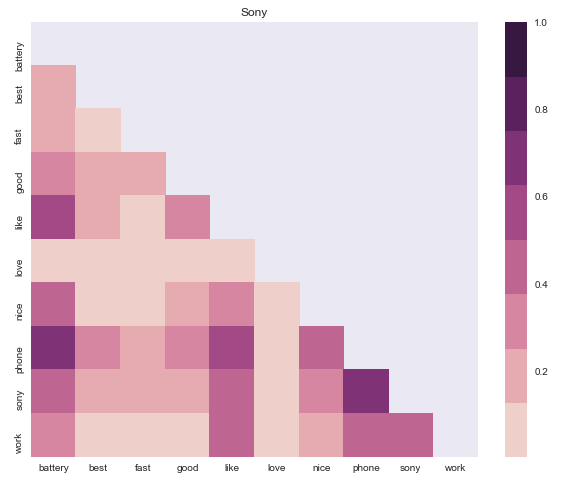
\includegraphics[width=\linewidth]{correlations.png}
  \caption{Correlations of the words with reviews}
  \label{fig:correlations}
\end{figure}

These was the basic analysis of the dataset. Further analysis is closely connected to the natural language processing and sentiment analysis, thus it will be explained into more details in the next section. 


\section{Methods}
We used two approaches to finding important features of cell phone brands. First is using supervised learning to classify new review as positive or negative, and after this we extract important words and do the sentiment analysis. Second approach ETC...


\subsection{Naive Bayes Classifier}

The reviews are split into positive and negative based on the ratings, and they are separately analysed. We decided to consider ratings four and five positive reviews, one and two as negative reviews. Reviews rated with three were not taken into account as we considered them to be neutral. After marking the reviews as positive, negative or neutral we used supervised learning to check if we will be able to train the model to predict if some new review is positive or negative. We used 90\% of the data for training and 10\% for the validation and with Naive Bayes Classifier we got result of ~84\% of successful classification. Most important features for the classifying the review as negative are words scam and false, whereas for classifying the review as positive important words are perfect and excelent. As the aim of our project is not to find only the important features, but to determine which of some specific features - like battery, ergonomy, screen, camera, etc - are correlated and important for some brands, we go further with the second step in the analysis. 
TODO: mention tokenize, lemmatization, stemming, stop words, etc. 


\subsection{Further sentiment analysis} 

Here we take sligthly modified approach. We undertake the next steps: 

 \begin{itemize}
  \item First we split the reviews according to the brand and according to the ratings - five groups are created for ratings from one to five.
  \item Next we do topic modelling using words vectors and Latent Dirichlet Allocation (LDA). Reviews are seen as a bag of words, and topics as a distribution over a fixed vocabulary. Words are generated from document specific topic distributions. As the output of this step we have 10 topics with 10 most import words for each topic (for each brand).
  \item After this we tag a sentiment on topic words. We use the previous Sentiment Analyzer to get a weighted sentiment for the topic. Here we consider two kind of words. First are feature words which we are mostly interested in - like battery or screen. Second group of words are non-feature words (great, bad, problem, work, etc). Non-feature words in the topic will be subject to sentiment analysis. 
  \item The weighted scores of all the non-feature words will be given to all the feature words in the following topic. If a topic does not contain feature words, it is ignored.
  \item At the end, we group the results to get an overview for all the reviews and all ratings. We count the density of appearence for each feature word in each topic. As a result and we show the sum of polarity scores for each feature word.
\end{itemize}


\section{Results and Findings}
From the exploratory analysis we can make next conclusions: The most reviewed model is ..., the highest mean prices has Apple, followed by .. 


\section{Conclusion}
This platform uses reviews and extracts meaningful information from it, and then evaluates certain cell phone brand based on these reviews. We use sentiment analysis to classify each of the reviews and it's parts as good or bad. After this process we find appeareances and sentiment for the feature words (for example battery, screen, camera, etc). Based on this we describe and evaluate specific brands. 


\begin{thebibliography}{}

\bibitem[\protect\citename{Aho and Ullman}1972]{Aho:72}
Alfred~V. Aho and Jeffrey~D. Ullman.
\newblock 1972.
\newblock {\em The Theory of Parsing, Translation and Compiling}, volume~1.
\newblock Prentice-{Hall}, Englewood Cliffs, NJ.

\bibitem[\protect\citename{{American Psychological Association}}1983]{APA:83}
{American Psychological Association}.
\newblock 1983.
\newblock {\em Publications Manual}.
\newblock American Psychological Association, Washington, DC.

\bibitem[\protect\citename{{Association for Computing Machinery}}1983]{ACM:83}
{Association for Computing Machinery}.
\newblock 1983.
\newblock {\em Computing Reviews}, 24(11):503--512.

\bibitem[\protect\citename{Chandra \bgroup et al.\egroup }1981]{Chandra:81}
Ashok~K. Chandra, Dexter~C. Kozen, and Larry~J. Stockmeyer.
\newblock 1981.
\newblock Alternation.
\newblock {\em Journal of the Association for Computing Machinery},
  28(1):114--133.

\bibitem[\protect\citename{Gusfield}1997]{Gusfield:97}
Dan Gusfield.
\newblock 1997.
\newblock {\em Algorithms on Strings, Trees and Sequences}.
\newblock Cambridge University Press, Cambridge, UK.

\end{thebibliography}

\end{document}
